% Using signed distance functions to embed contours in discrete grids
% Author: Josh Chang
\documentclass{article}
\usepackage{tikz}
\usetikzlibrary{positioning}
\usetikzlibrary{calc}
\usetikzlibrary{arrows,shapes,backgrounds}
\begin{document}
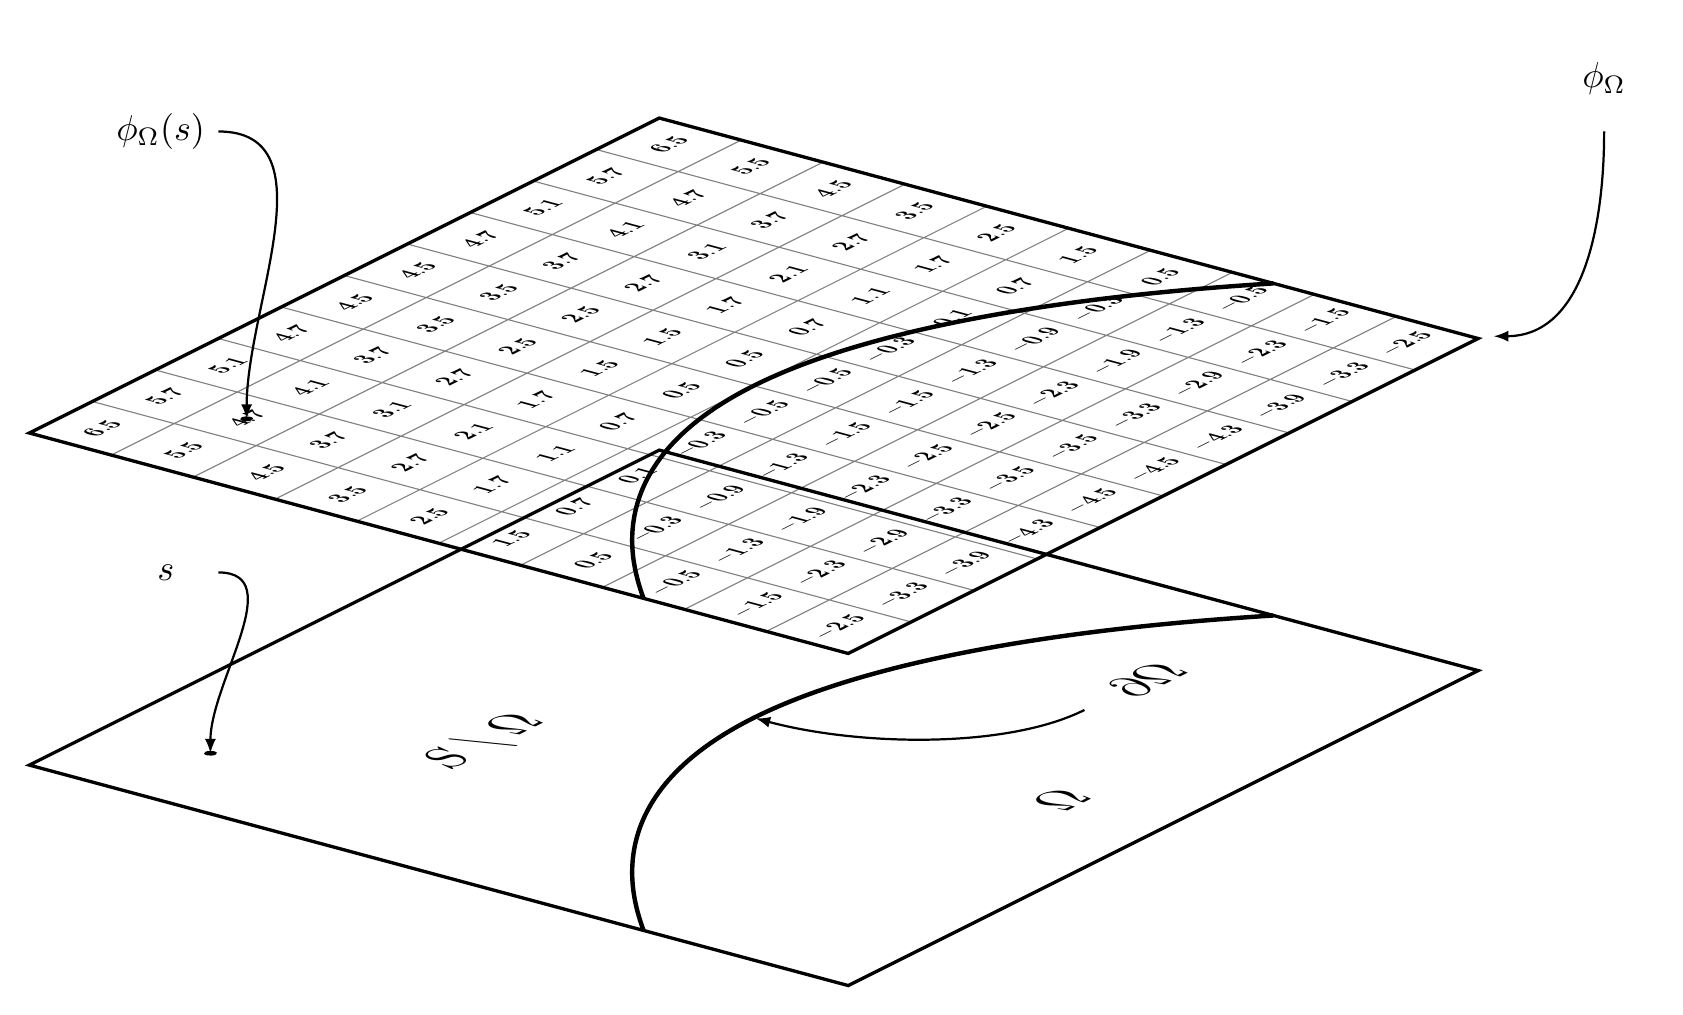
\begin{tikzpicture}[scale=2,every node/.style={minimum size=1cm},on grid]
		
    % slanting: production of a set of n 'laminae' to be piled up.
    % N=number of grids.
    \begin{scope}[
            yshift=-100,every node/.append style={
            yslant=0.5,xslant=-1.3},yslant=0.5,xslant=-1.3
            ]
        % opacity to prevent graphical interference
        \fill[white,fill opacity=0.9] (0,0) rectangle (4,4);
        \draw[step=4mm, thin, gray] (0,0) grid (4,4); %defining grids
        \draw[black,very thick] (0,0) rectangle (4,4);%marking borders      
        \draw [ultra thick](0,1) parabola bend (2,2) (4,1)  ; % parabola curve

\coordinate (sphi) at (0.6,3.4);
\node at (sphi) [fill=black,circle,scale=0.1] {$s$};

\pgfkeys{/pgf/number format/.cd, fixed, zerofill, precision =1} 

\foreach \x in {0,...,9} {
    \foreach \y in {0,...,9} {
%calculate the signed distance
%
% use newton raphson for 4 iterations to compute the distance
% 
        \pgfmathparse{0.2+0.4*\x}
        \pgfmathresult \let\xpoint\pgfmathresult;
        \pgfmathparse{0.2+0.4*\y}
        \pgfmathresult \global\let\ypoint\pgfmathresult;

        \pgfmathparse{\xpoint}
        \pgfmathresult \global\let\xx\pgfmathresult;
	% Run 4 iterations of Newton-Raphson to compute distance
          \foreach \iter in {1,...,4} {
              \pgfmathparse{0.25*(\xx*\xx*\xx-6*\xx*\xx+4*(\xx-2)*\ypoint
               +12*\xx-8*\xpoint+8)}
              \pgfmathresult \let\functionderv\pgfmathresult;
              \pgfmathparse{3*(\xx-2)*(\xx-2)/4+\ypoint}
              \pgfmathresult \let\functiondervv\pgfmathresult;
              \pgfmathparse{\xpoint-\functionderv/(\functiondervv)}
             \pgfmathresult \let\xx\pgfmathresult;
          }
          
          \pgfmathparse{-\xx*\xx/4+\xx+1}
          \pgfmathresult \global\let\yy\pgfmathresult;
          \pgfmathsetmacro{\dd}{sqrt((\xpoint-\xx)* (\xpoint-\xx)
            + (\ypoint-\yy)*(\ypoint-\yy ))/.4};
          \pgfmathparse{int(\yy*100)}
          \pgfmathresult \let\yyy\pgfmathresult;
          \pgfmathparse{int(\ypoint*100)}
          \pgfmathresult \let\yypoint\pgfmathresult;
          \ifnum \yyy > \yypoint { %% Signed distance
              \pgfmathparse{-\dd} \pgfmathresult \global\let\dd\pgfmathresult;
              }
          \fi	
         \node[scale=0.7,thick] at (\xpoint,\ypoint)
            {$\mathbf{\pgfmathprintnumber{\dd}}$};
     }
  }

    \end{scope}

    \begin{scope}[
        yshift=-160,every node/.append style={
        yslant=0.5,xslant=-1.3},yslant=0.5,xslant=-1.3
                  ]
        %marking border
        \draw[black,very thick] (0,0) rectangle (4,4);


        %draw bottom parabola
        \draw [ultra thick](0,1) parabola bend (2,2) (4,1)  ;
        \draw[-latex,thick](2.8,1)node[right,scale=1.5]{$\partial\Omega$}
                 to[out=180,in=270] (2,1.99);

\node at (2,0.5) [scale=1.5] {$\Omega$};
\node at (1.2,2.7) [scale=1.5] {$S\setminus\Omega$};
\coordinate (s) at (0.5,3.5);
\node at (s) [fill=black,circle,scale=0.1] {$s$};

    \end{scope} %end of drawing grids

% signed distance
\draw[-latex,thick](4.8,-.2)node[above,scale=1.3]{$\phi_\Omega$}
        to[out=-90,in=0] (4.1,-1.5);

% s
\draw[-latex,thick](-4,-.2)node[left,scale=1.3]{$\phi_\Omega(s)$}
        to[out=0,in=90] (sphi);

%s
  \draw[-latex,thick](-4,-3)node[left,scale=1.3]{$s$}
        to[out=0,in=90] (s);  	
\end{tikzpicture}
\end{document}
